%Einleitungstext zum Modul
\section{Klassen}
\graphicspath{{./img/settings/}}
Alle Klassen, die für die Funktionen benötigt werden, ohne spezifische Implementierungen zu nennen.
%Bild der Klasse aus dem Klassendiagramm (nur die Klasse jeweils)
%Dokumentation zur Klasse, öffentlichen Methoden und Konstruktor sowie:
%Signal und Slots als Methoden mit Rückgabewert Sigal bzw Slot (zur kenntlichkeit)
\subsection{CAlgorithmSettingController}
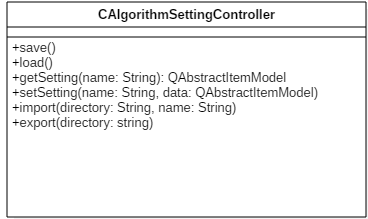
\includegraphics[scale=1, resolution=100]{CAlgorithmSettingController}\\
Verwaltet die Einstellungen der Algorithmen.
\beginMembers
\newMember{{getSetting}}{QString name}{CAlgorithmItemModel}{Gibt die aktuellen Parameter des Algorithmus "name" als ItemModel zurück.}
\newMember{{setSetting}}{QString name, CAlgorithmItemModel data}{bool}{Setzt die Parameter des Algorithmus "name"  gemäß dem ItemModel "data". true, falls erfolgreich, sonst false}
\newMember{{import}}{QUrl directory, QString name}{void}{Importiert die Datei "name" mit den Algorithmenparametern aus dem verzeichnis "directory".Die Datei muss im Json-Format vorliegen}
\newMember{{export}}{QUrl directory}{void}{Exportiert die Einstellungen aller Algorithmen in das Verzeichnis "directory".}
\closeMembers
\subsection{CGlobalSettingController}
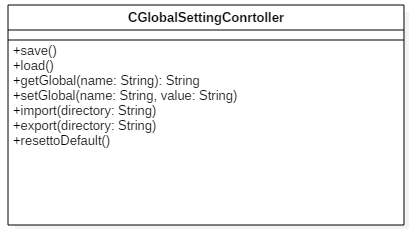
\includegraphics[scale=1, resolution=100]{CGlobalSettingController}\\
Verwaltet die globalen Einstellungen.
\beginMembers
\newMember{{getSetting}}{QString name}{QString}{Gibt die Einstellung "name" als QString zurück.}
\newMember{{setSetting}}{QString name, QString value}{bool}{Setzt den Wert "value" für die globalen Einstellung "name". true, falls erfolgreich, sonst false}
\newMember{{import}}{QUrl directory, QString name}{void}{Importiert die Datei "name" mit globalen Einstellungen aus dem Verzeichnis "directory".Die Datei muss im Json-Format vorliegen}
\newMember{{export}}{QUrl directory}{void}{Exportiert die globalen Einstellungen in das Verzeichnis "directory".}
\newMember{{resettoDefault}}{void}{void}{Stellt die Standardeinstellungen wieder her.}
\closeMembers
\subsection{QAbstractItemModel}
\includegraphics[scale=1, resolution=100]{qAbstractItemModel}\\
QT Interface für ItemModels.

\subsection{CAlgorithmSettingsModel}
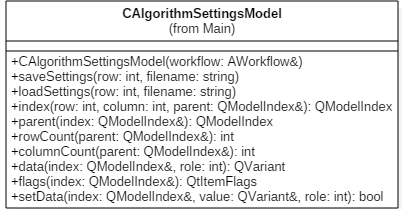
\includegraphics[scale=1, resolution=100]{CAlgorithmSettingsModel}\\
Implementierung des interfaces QAbstractItemModel.
\beginMembers
\newMember{{CAlgorithmSettingsModel}}{workflow:AWorkflow}{void}{ Konstruktor mit Workflow}
\newMember{{saveSettings}}{int row, String fielname}{void}{ Speichert eine Einstellung aus einer Reihe}
\newMember{{loadSettings}}{int row, String fielname}{void}{ Lädt eine Einstellung in eine Reihe}
\newMember{{index}}{int row, int column, QModelIndex parent}{QModelIndex}{Gibt einen Index von einem Item im Model zurück, abhängig von row, column und parent.}
\newMember{{parent}}{QMogelIndex index}{QModelIndex}{Gibt das parent von ItemModel mit dem index zurück}
\newMember{{rowCount}}{QModelIndex parent}{int}{Gibt die Reihe in Abhängigkeit von parent zurück}
\newMember{{columnCount}}{QModelIndex parent}{int}{Gibt die Spalte in Abhängigkeit von parent zurück}
\newMember{{data}}{QModelIndex index, int role}{Qvariant}{Gibt die gespeicherten Daten unter der role für das mit index referenzierte Item zurück}
\newMember{{flags}}{QModelIndex index}{QItemFlags}{Gibt die flag für index zurück}
\newMember{{setData}}{QModelIndex index, QVariant value, int role}{bool}{Setzt die Daten role für das Item index zu value. true, falls erfolgreich, sonst false}
\closeMembers
\section{Pakete}
Alle genannten Klassen liegen im Paket Settings.
%Einteilung der Teilmodule in Pakete 
%\subsection{Paket 1}
%Bild des Pakets mit vereinfachter Klassendarstellung
%Begründung / Dokumentation / Erklärung zum Paket
%\subsection{Paket 2}
%....
%\section{Entwurfsmuster}
% verwendete Entwurfsmuster aufzählen erklären etc mit verinfachtem Diagramm (Klassen ohne Inhalt nur die Namen)

\section{Klassendiagramm}
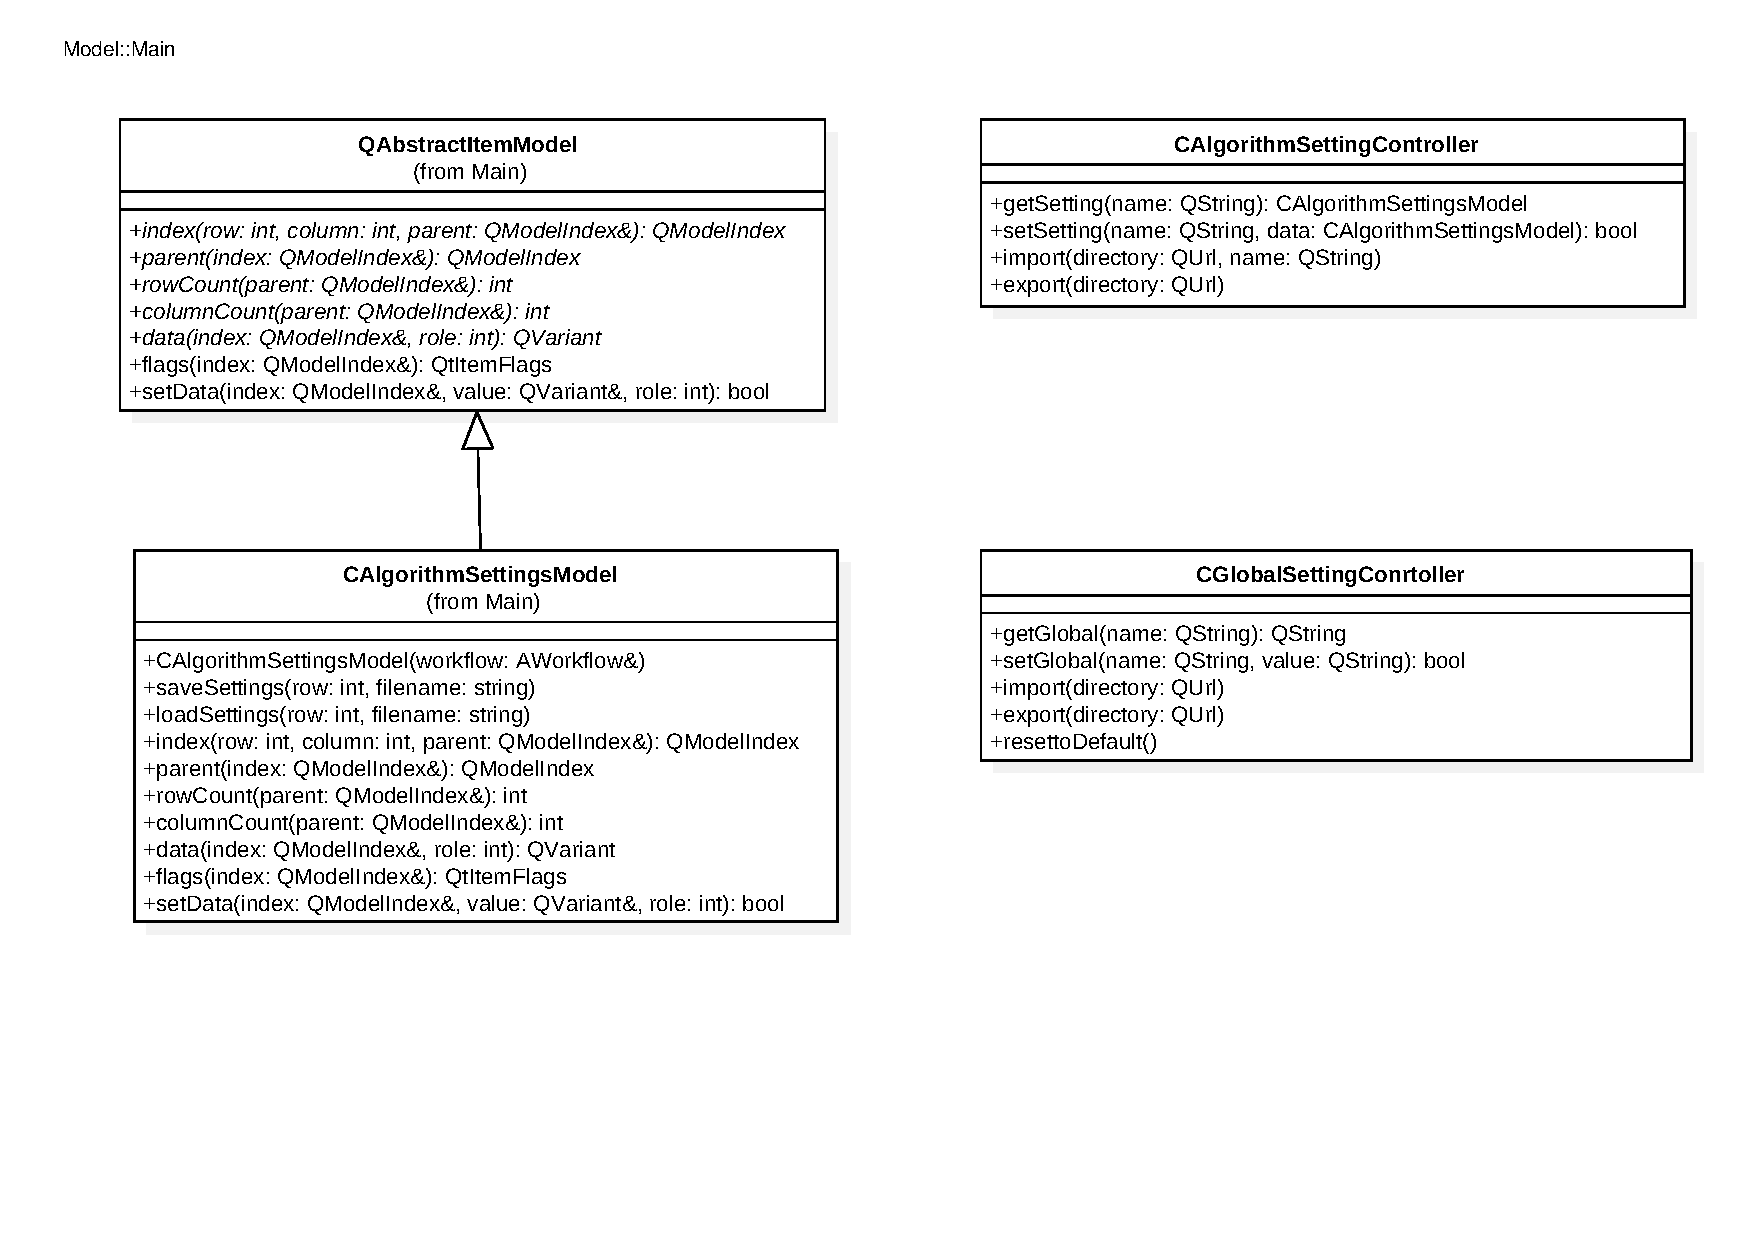
\includegraphics[width=\linewidth]{Settings}\\
% Klassendiagramm des Moduls

%Bitte jeweils kleine Einleitungstexte usw in Unterkapitel gerne auch in Textform Erklärungen zufügen und auf mögliche erweiterungen durch die kann Kriterien eingehen soweit nötig !